% Drawing 87/01-1 -- folder 87, batch 01, archive page 2 (PDF page 3).
% Transcription: à droite de ces formules, un croquis : une région $C$ hachurée par deux familles de droites parallèles. Le signe devant $\operatorname{bnd}_D$ est bien une intersection sur la page, là où l'on attendrait une réunion
% Kind: region hatched by two families of parallel lines. Method 2 (schematic redraw from the facsimile). Status: partial.
% Notes: A region crossed by two families of parallel lines (four or five lines each, drawn as straight strokes), a faint wavy outline around it and a brace on the left; two small ticks inside the region. The wavy outline is schematised; the label C is not on the sketch itself (it is in the formulas).
% Coordinates: 1 unit = 1 mm = 1/100 of the crop width (bbox in page fractions: [0.73, 0.585, 0.9, 0.67]).
% Redrawn by Claude (claude-opus-5-5), issue #73, 2026-11-07; not checked by a human; not compiled (no TeX in the session).
% Rights: reproduces part of the work -- behind RENDER_TRANSCRIPTS, never published by itself.
\documentclass[tikz,border=3pt]{standalone}
\usepackage{amsmath,amssymb}
\usetikzlibrary{patterns,arrows.meta}
\tikzset{pencil/.style={black!45}, struck/.style={black!35}, mark/.style={circle,draw,inner sep=1.3pt}, pt/.style={circle,fill,inner sep=0.9pt}, opt/.style={circle,draw,fill=white,inner sep=1.1pt}}
\begin{document}
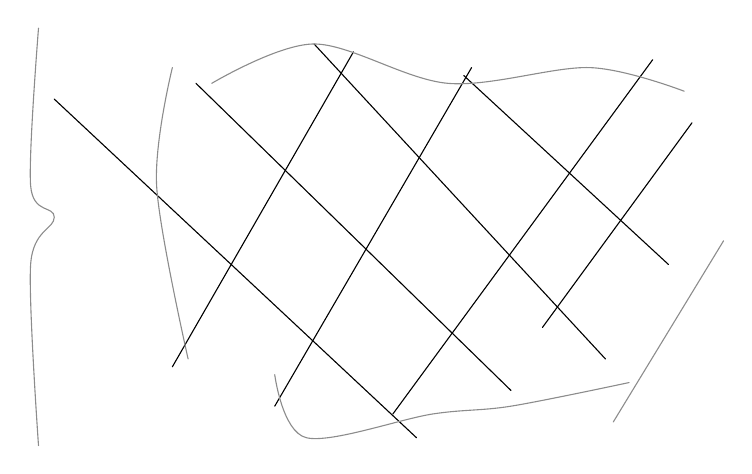
\begin{tikzpicture}[x=1mm,y=1mm,line cap=round,line join=round,font=\scriptsize]
\draw (12,-19) -- (58,-62);
\draw (30,-17) -- (70,-56);
\draw (45,-12) -- (82,-52);
\draw (64,-16) -- (90,-40);
\draw (27,-53) -- (50,-13);
\draw (40,-58) -- (65,-15);
\draw (55,-59) -- (88,-14);
\draw (74,-48) -- (93,-22);
\draw[pencil] (83,-60) -- (97,-37);
\draw[pencil] plot[smooth, tension=0.55] coordinates {(10,-10) (9,-30) (12,-34) (9,-40) (10,-63)};
\draw[pencil] plot[smooth, tension=0.55] coordinates {(27,-15) (25,-30) (29,-52)};
\draw[pencil] plot[smooth, tension=0.55] coordinates {(40,-54) (44,-62) (60,-59) (70,-58) (85,-55)};
\draw[pencil] plot[smooth, tension=0.55] coordinates {(32,-17) (45,-12) (62,-17) (80,-15) (92,-18)};
\end{tikzpicture}
\end{document}
